\chapter{Case Study: Benchmarking the Unipept Metagenomics Analysis Pipeline}
\chaptermark{Benchmarking the UMAP}
\label{chap:casestudy}

In dit hoofdstuk evalueren we de prestaties van de Unipept Metagenomics Analysis
Pipeline (UMAP). Dat werd onderzocht in een groepsproject van het vak
Computationele Biologie, gedoceerd door professor Dawyndt, door een groep van
vijf studenten (Robin Declerck, Simon Houbracken, Michael Niklaus, Ine
Melckenbeeck, Bereket Tesfamariam Habtemariam) onder leiding van mijzelf.

In een tweede project binnen het vak werden, onder leiding van Felix Van der
Jeugt, reeds geclassificeerde peptiden in de IGC databank opnieuw
geclassificeerd met de UMAP. Zij concludeerden dat het grootste deel van de
resultaten overeen kwamen tussen Unipept en IGC, maar dat Unipept meer (zowel
true als false) positives rapporteert en daarenboven ook een specifieker
onderscheid tussen de verschillende rangen maakt. Het volledige onderzoek is te
lezen in de scriptie: ``Optimaliseren van de Unipept Shotgun
Metaproteomics Analysis Pipeline''\cite{felixthesis}.

Ter herhaling doorloopt de UMAP enkele stappen, geïllustreerd in de inleiding in
\Vref{fig:van_naar}. Voor elke DNA read in een metagenomics sample kunnen we een
proteomics experiment doen. Hierbij zoeken we, bijvoorbeeld aan de hand van
FragGeneScan, alle eiwitten op de DNA read in kwestie. De bekomen eiwitten
worden opgedeeld in tryptische peptiden waarna elke peptide afzonderlijk op zijn
taxonomische identificatie wordt afgebeeld door middel van het lowest common
ancestor (LCA) algoritme. Aan de hand van het LCA* algoritme, beschreven in
\Vref{chap:lca*}, kunnen we de bekomen taxa aggregeren naar een
consensusclassificatie.

Voor dit benchmarkingsproces gaan we eerst op zoek naar een manier om te testen
hoe goed de UMAP presteert op ongekende data en stellen we een aantal kernvragen
die binnen dit onderzoek beantwoord moeten worden. Daarna worden de genomen
stappen in het onderzoek besproken en vatten we de resultaten samen. ``Goed
presteren'' definiëren we hier aan de hand van één hoofdzaak en enkele bijzaken.
De toolchain moet hoofdzakelijk een zo specifiek mogelijke, maar wel correcte,
identificatie van de invoerdata als resultaat geven. Daarnaast moet de
identificatie ook snel kunnen gebeuren zonder al te veel hardwarebenodigdheden
te vragen.

\section[Bepalen van een benchmarkstrategie]{Bepalen van een benchmarkstrategie%
  \sectionmark{Benchmarkstrategie}}
\sectionmark{Benchmarkstrategie}

Het bepalen van een benchmarkstrategie is cruciaal om tot betrouwbare resultaten
te komen. Op het eind van deze case study willen we drie vragen kunnen
beantwoorden: \textit{i)} hoe accuraat is taxonomische identificatie met de
UMAP, \textit{ii)} hoe accuraat is die taxonomische identificatie wanneer ze
wordt toegepast op onbekende data en \textit{iii)} hoe goed presteert de UMAP op
gesimuleerde DNA reads die fouten bevatten?

De eerste vraag kunnen we onderzoeken door bekende, volledig gesequeneerde
genomen als invoer van de UMAP te gebruiken. Aangezien alle data uit deze
genomen bekend is, en we er ook van uit gaan dat de taxonomische identificatie
van de genomen correct is, verwachten we dat de resultaten zeer specifiek zullen
zijn.

De tweede vraag is echter moeilijker te beantwoorden. We kunnen namelijk geen
analyse uitvoeren van nog niet gesequeneerde genomen, aangezien we dan geen
objectieve manier hebben om in te schatten hoe accuraat het resultaat van de
analyse zou zijn. Wat we wel kunnen, is dit soort genomen simuleren op basis van
de complete genomen uit de vraag hierboven. Wanneer we de \Vref{fig:workflow} er
nog eens bij halen, zien we dat in de Unipept Metaproteomics Analysis Pipeline
de LCA van een peptide wordt berekend aan de hand van de eiwitten waarin dit
peptide voorkomt. Deze eiwitten worden dan afgebeeld op hun overeenkomstige
taxa, waarna via een aggregatie via LCA een consensustaxon bekomen wordt. Stel
nu echter dat een genoom, en bij gevolg ook eiwitten uit dat genoom, niet
gekend is, dan zal de resulterende mapping van een peptide naar eiwitten die
eiwitten ook niet bevatten. Het proces van ``niet gekend zijn'' kunnen we dus
simuleren door alle eiwitten die voorkomen in het oorspronkelijk genoom te
schrappen uit de lijst van eiwitten bij een peptide horen. Door middel van deze
filterstap (soort van leave-one-out strategie) kunnen we dus een ongekend genoom
simuleren uit een wel gekend genoom en kunnen we toch nog de resultaten
vergelijken.

De derde vraag kan op de volgende manier beantwoord worden. We kunnen aan de
hand van een read simulator, zoals wgsim \cite{lh3/w4:online}, reads met
verschillende error percentages simuleren op basis van een volledig genoom. In
deze reads kunnen we dan via een gene predictor, bijvoorbeeld FragGeneScan
\cite{rho2010fraggenescan}, eiwitfragmenten extraheren. Op deze eiwitten kunnen
we kunnen we dan de UMAP uitvoeren en de resultaten vergelijken met de
resultaten van de UMAP op het originele genoom.

We werken dus twee benchmarks uit. In de eerste nemen we de sequentie van een
genoom als invoer, waaruit we alle eiwitten extraheren. Die eiwitten splitsen
we vervolgens op in peptiden, waarop de Unipept Metaproteomics Analysis Pipeline
wordt uitgevoerd. De resulterende lijst van taxa aggregeren we nu per proteïne
met het LCA* algoritme naar een consensustaxon. Als uitvoer krijgen we dan voor
elke proteïne in het invoergenoom een taxonomische identificatie die we kunnen
vergelijken met de taxonomische identificatie van het genoom zelf. Deze
toolchain noemen we in het vervolg \texttt{pept2lca2lca*}. De naamgeving hiervan
steunt op de genomen stappen in de analyse: van peptiden $\rightarrow$ lca en
van lca $\rightarrow$ lca*. In de volgende sectie zal deze naamgeving
verduidelijkt worden.

Bij de tweede toolchain nemen we opnieuw een genoom als invoer, waaruit we
opnieuw alle eiwitten extraheren. De eiwitten splitsen we op in peptiden. Deze
peptiden verwerken we op vergelijkbare wijze als hierboven, maar nu met een
bijkomende tussenstap. Voor elke peptide wordt eerst een lijst van eiwitten
opgevraagd waar het betreffende proteïne in voorkomt. Uit deze lijst worden dan
de eiwitten gefilterd die reeds voorkomen in het invoergenoom. De resterende
eiwitten worden verder verwerkt door ze af te beelden op hun taxa in de Unipept
taxonomie, waarna ze worden geaggregeerd via het LCA algoritme. De lijst van
resulterende taxa wordt vervolgens per proteïne geaggregeerd wordt de lijst van
resulterende taxa per proteïne geaggregeerd met het LCA* algoritme, wat een
zelfde lijst als bij de eerste toolchain oplevert. Naar deze toolchain verwijzen
we vanaf nu met \texttt{pept2prot2filter2lca}, steunend op de overgangen van
peptiden $\rightarrow$ eiwitten, eiwitten $\rightarrow$ gefilterde eiwitten,
gefilterde eiwitten $\rightarrow$ lca*.

Door één invoergenoom op beide manieren te verwerken, krijgen we nu één
consensustaxon per proteïne uit het genoom. Deze twee lijsten kunnen we nu
onderling vergelijken om na te gaan hoeveel er precies aan specificatie verloren
is gegaan door de filterstap. Voor een goede taxonomische identificatie door
UMAP verwachten we dat de eerste lijst (zonder filtering) bijna volledig zal
bestaan uit taxa op \textit{species} niveau. De tweede lijst (analyse op
gesimuleerde onbekende genomen) kunnen we dan vergelijken met de eerste lijst om
het verlies aan taxonomische identificatie in te schatten wanneer er wordt
gewerkt met ongekende genomen.

Op deze twee resulterende lijsten van taxa wordt ook een onderscheid gemaakt
tussen specificatieverlies en een verkeerde identificatie van een taxon. Wanneer
het resulterende taxon op de lineage ligt van het taxon van het genoom in de
invoer, maar niet van de rang \textit{species} is, verliezen we aan
specificatie. Dit zullen we aangeven met de term ``match''. Wanneer de
resulterende taxon niet op de lineage ligt van het taxon van het ingevoerde
genoom, spreken we van een verkeerde identificatie, of ``mismatch''.

Als invoer voor dit benchmarkingsproces gebruiken we een lijst van ruim duizend
volledig gesequeneerde genomen uit de NCBI databank. Beide toolchains worden
geïllustreerd in \Vref{fig:abstractimage}.

\begin{figure}
	\centering
	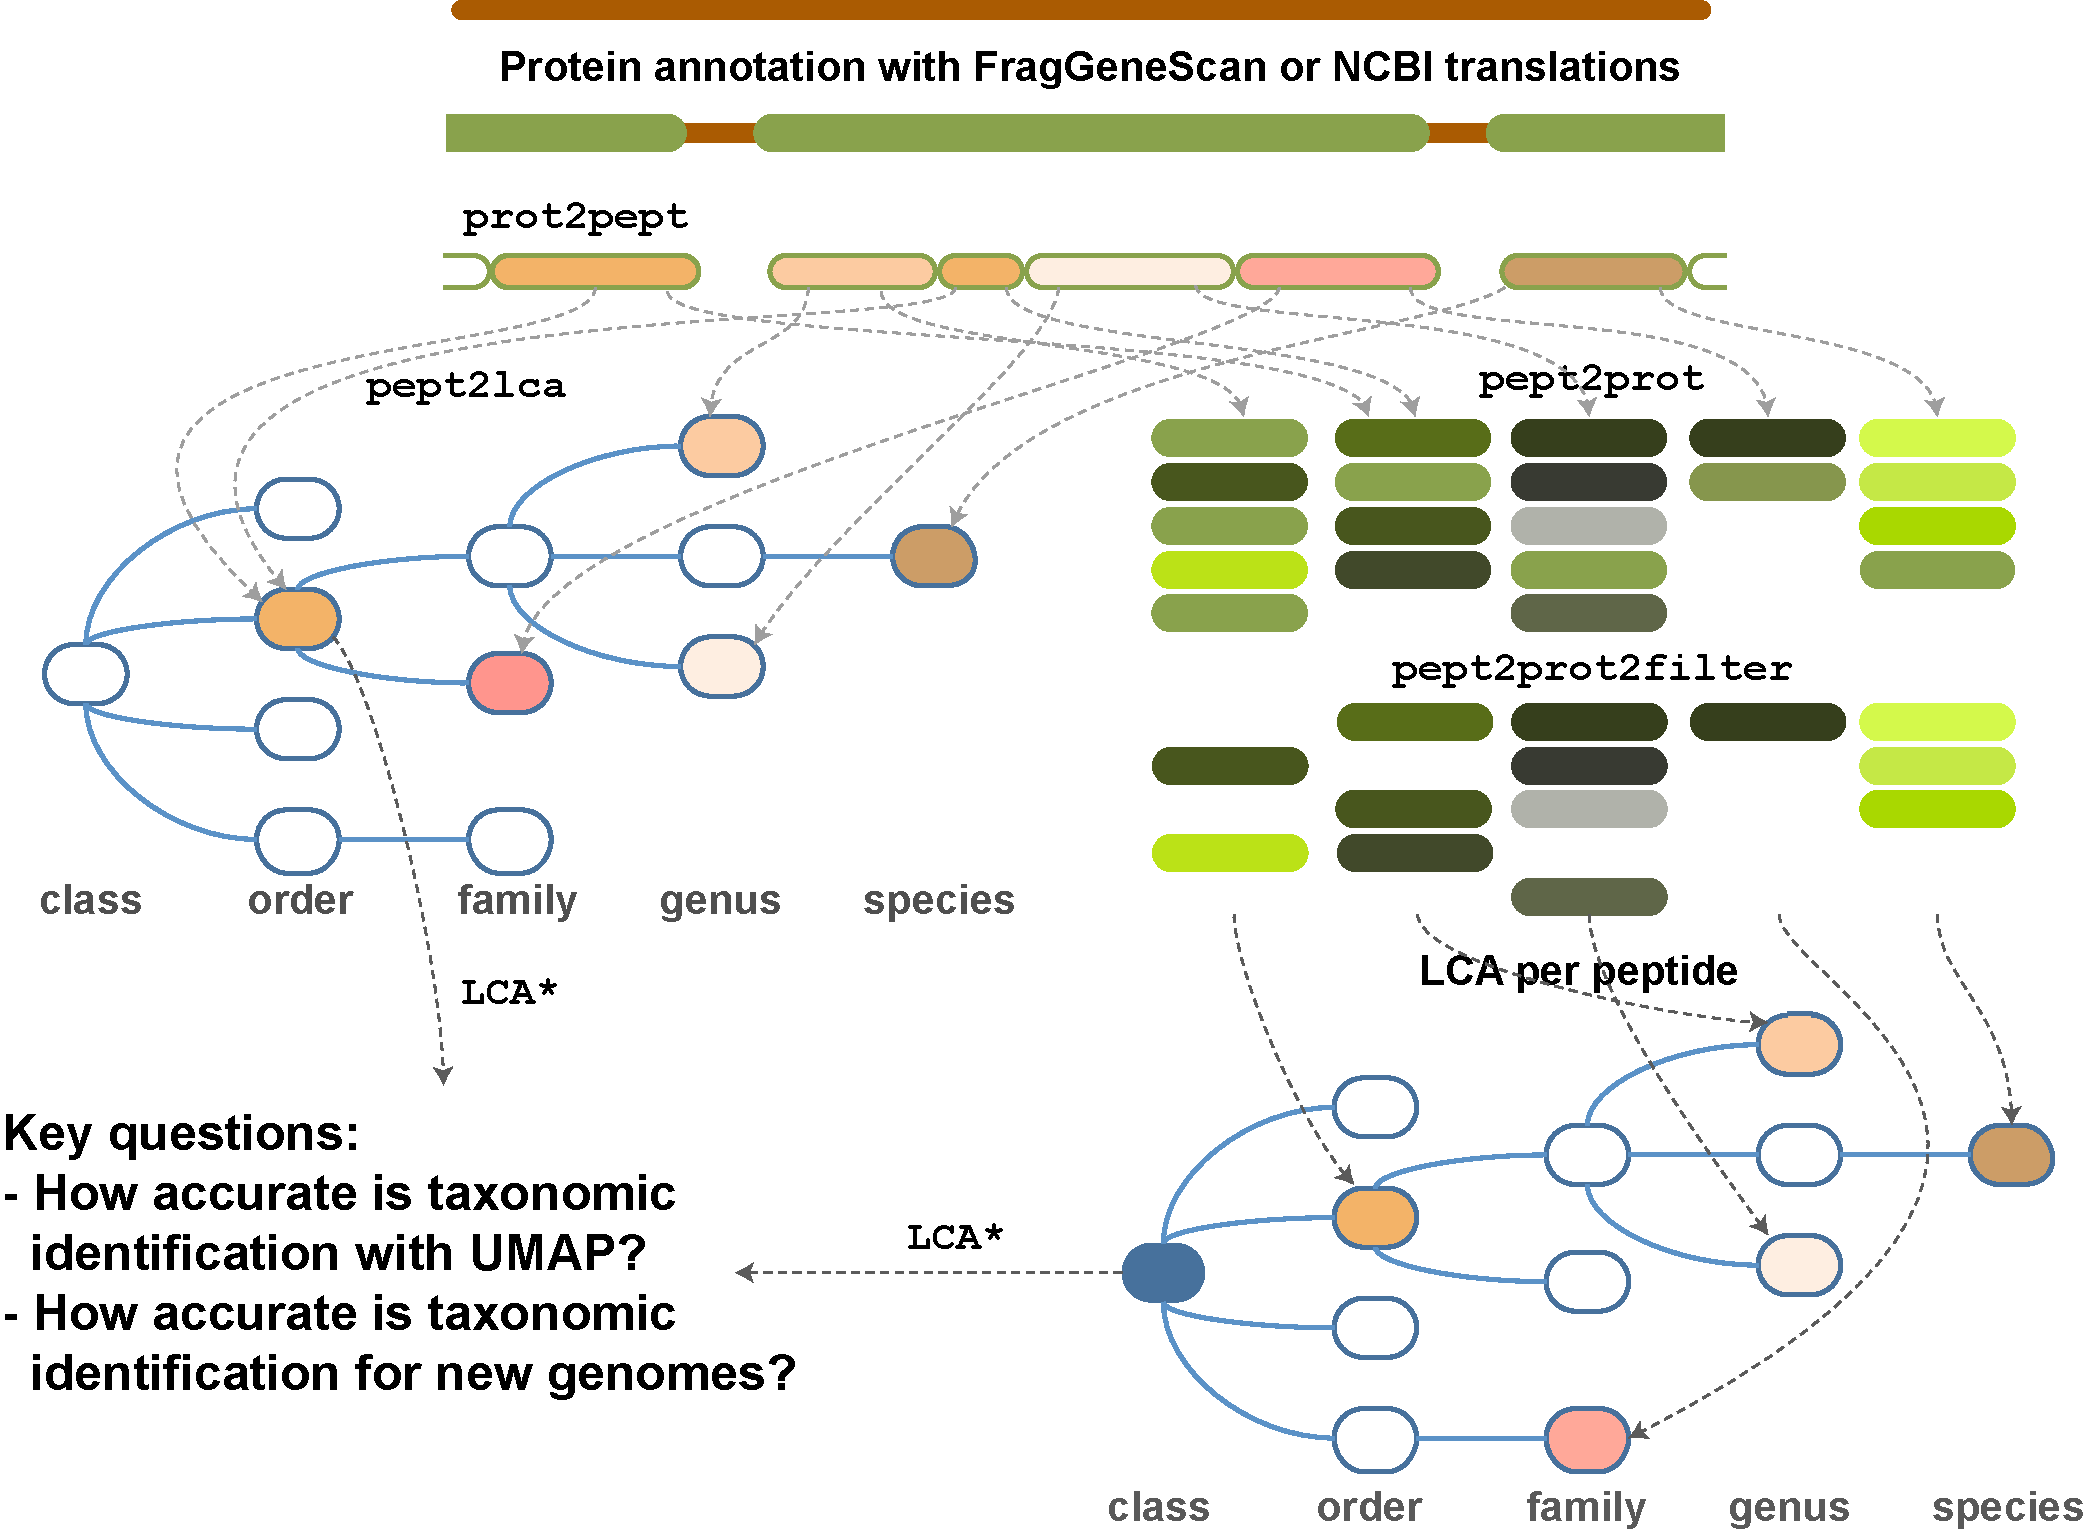
\includegraphics[width=0.8\textwidth]{includes/abstractimage.pdf}
	\caption{Illustratie van beide processen. Alle eiwitten worden uit een 
	genoom geëxtraheerd en opgesplitst in peptiden. Die peptiden worden dan 
	verwerkt via de Unipept Metaproteomics Analysis Pipeline tot taxa (links) 
	of worden (rechts) verwerkt door eerst alle eiwitten op te vragen waarin 
	de peptide voorkomt. Daarna wordt die lijst van eiwitten gefilterd op 
	eiwitten die voorkomen in het originele genoom. Vervolgens worden die 
	eiwitten afgebeeld via LCA op hun consensustaxa in de Unipept taxonomie. 
	Beide resulterende lijsten van taxa worden dan door een LCA* stap per 
	proteïne geaggregeerd en met elkaar vergeleken.}
	\label{fig:abstractimage}
\end{figure}

\section{Implementatie} 

De implementatie van de twee hierboven beschreven toolchains steunt op een 
aantal tools en bibliotheken. In deze sectie bespreken we eerst
deze lijst en geven we aan waar we de tools voor gebruiken. Daarna volgt de
bespreking van het benchmarkingsproces aan de hand van een analysescript.
Vervolgens staan we nog stil bij een ingreep in dat script om de snelheid ervan
te verhogen.

\subsection{Gebruikte tools en bibliotheken}

\begin{itemize}

\item \textbf{Unipept-CLI:} zoals beschreven in de inleiding is de Unipept-CLI
een interface in Ruby naar de webservices van Unipept. Hiermee kunnen alle
methodes van de Unipept webservices aangesproken worden. We maken gebruik van de
commando's \texttt{pept2lca}, die een lijst van peptides op hun LCA afbeeldt, en
\texttt{pept2prot} die voor een peptide een lijst van eiwitten oplevert waar
die peptide in voorkomt. Met de Ruby \texttt{unipept}-gem komen ook de
commando's \texttt{prot2pept}, die een een proteïne omzet in tryptische
peptides, en \texttt{peptfilter} die te lange (>50) of te korte (<5) peptides
filtert uit een lijst van opgegeven peptides.

\item \textbf{Biopython:} Biopython \cite{Biopy8:online} is een Python 
bibliotheek die een heel aantal tools voor computationele biologie bundelt. Wij 
zullen gebruik maken van de Entrez module \cite{Bio.E7:online}. Deze module 
zorgt ervoor dat we via de command-line toegang hebben tot de NCBI database om 
bijvoorbeeld alle eiwitten uit een genoom op te vragen.

\item \textbf{UniProt mapping:} De UniProt mapping \cite{Retri1:online} service
is een webservice die het vertalen van identifiers van eiwitten van en naar
overeenkomstige identifiers uit verschillende databanken vereenvoudigt. Deze
worden specifiek gebruikt om de identifiers van proteïne uit NCBI om te zetten
naar UniProtKB identifiers.

\item \textbf{RMQ-bibliotheek:} Een implementatie van een RMQ library
\cite{Hideo0:online, Hideo1:online} in C die voldoet aan de besproken snelheids-
en ruimtecomplexiteiten uit \Vref{chap:lca*}.

\item \textbf{Eigen scripts:} Deze scripts kunnen worden onderverdeeld in twee 
soorten:

    \begin{itemize}
    
    \item Een reeks van \textbf{wrapper scripts} in Bash en Python die hierboven
    benoemde tools wrappen. Deze zijn gemaakt om bijvoorbeeld alle eiwitten op
    te vragen van een NCBI assembly of bijvoorbeeld om het resultaat van de
    \texttt{pept2lca} stap te aggregeren via LCA*, gebruik makend van de
    RMQ-bibliotheek.
    
    \item \textbf{Ondersteunende scripts} die de volledige taxonomische boom
    inladen en aan de hand van die data de benodigde arrays voor de
    preprocessing van RMQ opstellen.
    \end{itemize}

\end{itemize}

\subsection{Implementatie van de benchmark} 

In dit gedeelte overlopen we een analysescript in Bash, dat alle stappen van het
volledige benchmarkingsproces uitvoert. De enige parameter waarmee dit script
moet worden aangeroepen is een GenBank accession number van een assembly. Dit
ziet er bijvoorbeeld uit als \texttt{GCA\_000015425.1}.
\begin{lstlisting}[language=Bash]
#!/bin/bash
asm_id=$1 && shift
\end{lstlisting}

Aangezien alle scripts verspreid staan over meerdere folders en we ook een
aantal (tussentijdse) resultaten wegschrijven, stellen we eerst enkele folders
in en maken we die aan waar nodig. De gebruiker kan kiezen om de
standaardwaarden van die folders te overschrijven aan de hand van opties van het
Bash script.

\begin{lstlisting}[language=Bash,firstnumber=3]
# Save directory of the analysis script to know where to find the others
dir="$(dirname "$0")"

# Create a tmpdir and a datadir
tmpdir=$(mktemp -d -t "$asm_id.XXXXXXXXXX")
datadir=$tmpdir
rmqdatadir=""

while getopts "d:t:r:" opt
do
  case $opt in
    d)
      datadir="$OPTARG/$asm_id"
      ;;
    t)
      tmpdir="$OPTARG/$asm_id"
      ;;
    r)
      rmqdatadir="-r $OPTARG"
      ;;
    ?)
      usage
      ;;
  esac
done

mkdir -p $datadir
mkdir -p $tmpdir

echo "Writing data to $datadir"
echo "Writing tempdata to $tmpdir"
\end{lstlisting}

De eerste stap is het ophalen van de taxon identifier van de assembly. Dit 
gebeurt aan de hand van het \texttt{asm2taxid} script, dat een wrapper is rond 
de Entrez module in BioPython. Het resultaat hiervan is bijvoorbeeld 400667 
voor genoemd GenBank accession number 

\begin{lstlisting}[language=Bash,firstnumber=34]
# get the taxon ID of the assembly
tax_id=$(python3 $dir/../entrez/asm2taxid.py $asm_id)
\end{lstlisting}

We moeten natuurlijk ook alle peptiden hebben als brondata voor een analyse. Dit
doen we aan de hand van het wrapperscript \texttt{asm2pept} dat, gegeven een
assembly identifier, de bijhorende eiwitten uit de NCBI databank opvraagt en
die eiwitten via de commando's \texttt{prot2pept} en \texttt{peptfilter} omzet
naar een lijst van peptiden. Deze peptiden worden gegroepeerd onder het id van
hun bijhorende proteïne opgeslagen in een FASTA bestand, genaamd
\texttt{peptides.fst}.

\begin{lstlisting}[language=Bash,firstnumber=36]
#  get the complete sequence and process it with:
#     - prot2pept
#     - peptfilter

echo "Getting peptides"
if [ ! -s "$tmpdir/peptides.fst" ]
then
  echo "No peptides found, downloading."
  python3 $dir/../entrez/asm2pept.py $asm_id > "$tmpdir/peptides.fst"
fi
\end{lstlisting}

Eens we de FASTA file van peptiden gegroepeerd hebben onder hun proteïne
identifier, kunnen we de eerste toolchain (de taxonomische identificatie
van volledige genomen) starten door \texttt{pept2lca} op dit bestand uit te
voeren. \texttt{pept2lca} vraagt aan de Unipept webservices voor elke peptide
zijn bijhorende taxonomische identificatie op. Het commando zorgt er ook voor
dat alles gegroepeerd blijft onder zijn FASTA header.

De uitvoer hiervan wordt naar het \texttt{pept2lca2lca} (vandaar ook de naam van
deze toolchain) commando gepiped. Het \texttt{pept2lca2lca} script is een
wrapperscript rond de RMQ-bibliotheek die voor de groepen van taxa onder een
proteïn identifier de LCA* berekent. Als optioneel argument neemt dit script een
taxon identifier. Wanneer deze taxon identifier wordt meegeleverd, voegt het
script een extra kolom toe aan de uitvoer die een 1 bevat wanneer resulterende
taxon een ``match'' is en 0 bevat wanneer de resulterende taxon een ``mismatch''
is.

De uitvoer wordt geschreven naar \texttt{pept2lca2lca.fst} wat het eindresultaat
is van de eerste toolchain.

\begin{lstlisting}[language=Bash,firstnumber=46]
# analyse the complete sequence with and
# check whether resulting taxa come from the correct lineage
#     - pept2lca2lca

echo "Executing pept2lca2lca"
unipept pept2lca -i "$tmpdir/peptides.fst" \
  | tee "$datadir/pept2lca.fst" \
  | python3 $dir/../pept2lca2lca.py -c $tax_id $rmqdatadir \
  > "$datadir/pept2lca2lca.fst"
\end{lstlisting}

De tweede toolchain vraagt een extra stap. Eerst worden aan de hand van het
wrapper script \texttt{asm2seqacc} rond de Entrez module alle identifiers van
sequences van een assembly opgevraagd. Deze worden vervolgens gepiped naar de
UniProt translation service om de UniProt identifier van deze eiwitten te
bekomen (hetgeen nodig is omdat we deze eiwitten later willen filteren).

Wegens een recente aanpassing van UnitProtKB waarbij alle redundante eiwitten
zijn verwijderd en samengevoegd \cite{Uniprotredun:online}, is het mogelijk
dat de vertaalservice een leeg antwoord teruggeeft. Zonder deze identifiers
kunnen we geen filtering doen, en is deze toolchain dan ook overbodig. Dit
blijkt het geval te zijn in ongeveer $27$\% van de assemblies. Voor de gevallen
waar het wel slaagt gaan we verder met de toolchain.

\begin{lstlisting}[language=Bash,firstnumber=55]
echo "Getting uniprot ids"
# get the proteins uniprot ids which occur in the genome
if [ ! -s "$tmpdir/uniprot_protein_ids.txt" ]
then
  echo "No uniprot ids found, downloading."
  python3 $dir/../entrez/asm2seqacc.py $asm_id \
  | python3 $dir/../entrez/seqacc2protid.py \
  > "$tmpdir/uniprot_protein_ids.txt"

  # Check if the file is still empty; no translation could be found.
  if [ ! -s "$tmpdir/uniprot_protein_ids.txt" ]
  then
    echo "ERROR: It seems that the uniprot_protein_ids.txt file is still empty. 
    Pept2prot2filter has no use anymore now." >&2
    exit
  fi
fi
\end{lstlisting}

De laatste stap in de \texttt{pept2prot2filter2lca} toolchain is het uitvoeren
van enkele wrapper scripts. We voeren eerst het \texttt{pept2prot} commando van
de \texttt{unipept} gem uit om alle eiwitten, behorend bij een peptide op te
vragen. Daarna pipen we deze lijst door naar \texttt{pept2prot2filter} die op
basis van de UniProt identifiers -- die in de vorige stap werden opgehaald -- de
eiwitten uit de lijst filtert die voorkomen in het originele genoom. Als laatste
voeren we nog de aggregatiestap uit. In deze stap worden eerst alle taxa
behorend bij één enkele peptide geaggregeerd, daarna worden die taxa ook nog
eens via het LCA* algoritme per proteïne identifier geaggregeerd. Ook
dit script neemt als parameter de taxon identifier van het origineel genoom om
``matches'' en ``mismatches'' te kunnen identificeren. Het resultaat komt
terecht in het bestand \texttt{pept2prot2filter2lca.fst}.

\begin{lstlisting}[language=Bash,firstnumber=72]
#     - pept2prot2filter2lca
echo "Executing pept2prot2filter2lca"
unipept pept2prot -i "$tmpdir/peptides.fst" \
  | $dir/../pept2prot2filter.sh "$tmpdir/uniprot_protein_ids.txt" \
  | python3 $dir/../pept2prot2filter2lca.py -c $tax_id $rmqdatadir \
  > "$datadir/pept2prot2filter2lca.fst"
\end{lstlisting}


\subsection{Snelheidsoptimalisatie}
\label{sec:snelheidsoptimalisatie}

Nu we van beide toolchains een resultaat hebben, kunnen we deze beginnen te
analyseren. De laatste stap in de tweede toolchain, en dan voornamelijk het
commando \texttt{pept2prot} duurt echter heel lang. Voor 3300 eiwitten kan dit
al snel enkele uren duren. De reden hiervoor is dat sommige peptiden zeer
universeel zijn en dus in heel erg veel eiwitten voorkomen. Het peptide
\texttt{IEELR} komt bijvoorbeeld in 162.827 eiwitten voor. Het 
\texttt{pept2prot}
commando uitvoeren op 72.888 peptiden (1.1MB) resulteert bijvoorbeeld in een
bestand van 64.949.837 lijnen ter grootte van 2.5GB. Dit is niet alleen 2.5GB
die wordt gedownload van de Unipept server, maar ook 2.5GB aan data die de
Unipept server zelf moet verwerken.

We kunnen dit optimaliseren volgens de volgende observatie. Stel dat we een
genoom analyseren met de tweede toolchain waar de peptide \texttt{IEELR} een
aantal keer in voorkomt. Dit zal alle 162.827 eiwitten ophalen. Wanneer we de 
bijhorende taxa bij de eiwitten aggregeren tot een consensustaxon zonder de 
filterstap zal de consensusclassificatie waarschijnlijk altijd in de minder 
specifieke rangen liggen, aangezien de peptide zo universeel voorkomt.

Wanneer we de filterstap wel uitvoeren en dus alle eiwitten van het originele
genoom uit deze lijst van 162.827 eiwitten filteren, zullen er nog steeds heel
veel van deze eiwitten overblijven en zal de aggregatie van hun bijhorende taxa
nog steeds een weinig specifiek resultaat opleveren. We kunnen met andere
woorden de eiwitten die universeel zijn tijdelijk uit de dataset halen zodat ze
niet worden meegerekend in de \texttt{pept2prot} stap. Na deze stap voegen we de
uitgefilterde eiwitten terug bij het eindresultaat en gaan we verder met de
toolchain.

Een benchmark van deze methode op de assembly met accession
\texttt{GCF\_000015425.1} voor \textit{Acinetobacter baumannii} ATCC 17978,
waarbij alle rangen boven family als universeel aanzien werden, resulteert in
een zeer kleine shift van ongeveer 1.5\% op van de hogere naar de lagere rangen.
Dit wordt geïllustreerd in \Vref{fig:leaveoneout}. Het resultaat van
\texttt{pept2prot} werd hiermee gereduceerd van 64.949.837 naar 21.794.027
lijnen en leverde een tijdwinst van ongeveer 300\% op.

\begin{figure}
	\centering
	\includegraphics[width=0.8\textwidth]{includes/leaveoneout}
	\caption{Benchmark om te testen wat het effect is van de 
	snelheidsoptimalisatie beschreven in \Vref{sec:snelheidsoptimalisatie}. Bij 
	de ``full search'' doen we de tweede toolchain met alle eiwitten. ``pruned 
	search'' laat voor de \texttt{pept2prot} stap alle universele peptiden weg  
	en voegt ze na de \texttt{pept2prot} stap terug toe.}
	\label{fig:leaveoneout}
\end{figure}

Aangezien deze snelheidsoptimalisatie een gigantische tijdwinst oplevert met een
minimaal effect op de identificatie, zullen we voor alle benchmarks gebruik
maken van deze snelle methode. De nieuwe code voor de tweede toolchain passen we
dan aan naar de volgende code. Hier splitsen we het \texttt{peptides.fst} op in
universele en niet-universele peptiden. Dit onderscheid wordt voor elke peptide
gemaakt aan de hand van de rang van zijn consensustaxon in het
\texttt{pept2lca.fst} bestand. Daarna voeren we op de gefilterde lijst het
\texttt{pept2prot} commando uit, waarna we de lijsten terug samenvoegen en
verder gaan met de toolchain.

\begin{lstlisting}[language=Bash, firstnumber=72]
#     - pept2prot2filter2lca
echo "Executing pept2prot2filter2lca"

# Divide peptides in universal and non-universal peptides
cat "$tmpdir/peptides.fst" \
  | python3 $dir/../commonpeptfilter.py "$datadir/pept2lca.fst" 
  "$tmpdir/peptides.filteredout.fst" > "$tmpdir/peptides.filtered.fst"

# Run pipeline
unipept pept2prot -i "$tmpdir/peptides.filtered.fst" \
  | $dir/../pept2prot2filter.sh "$tmpdir/uniprot_protein_ids.txt" \
  | {
    read -r hdr;
    echo $hdr;
    sort -m - "$tmpdir/peptides.filteredout.fst" \
      | python3 $dir/../pept2prot2filter2lca.py -c $tax_id $rmqdatadir \
      > "$datadir/pept2prot2filter2lca.fst"
    }
\end{lstlisting}

\section{Resultaten} 

In deze sectie bespreken we de resultaten en beantwoorden we de drie vragen die
in het begin van dit hoofdstuk gesteld werden. We bespreken eerst de resultaten
van beide toolchains toegepast op het genoom, \textit{Acinetobacter baumannii}
ATCC 17978 en bekijken ook het effect van de analyse na het simuleren van reads
op dit genoom. Daarna kijken we naar de resultaten van alle 1145 geanalyseerde
genomen voor beide toolchains en bestuderen we het effect van de analyse op
gesimuleerde onbekende genomen. Als laatste bekijken we de resultaten in een PCA
plot en bespreken we enkele outliers.

In \Vref{fig:barchart} staan de resultaten op het genoom van
\textit{Acinetobacter baumannii} ATCC 17978 van beide toolchains in een barchart
weergegeven. Op \Vref{tbl:barcharttable} staat de overeenkomstige tabel met
cijfers. Hierbij worden de resulterende taxa per rang proportioneel weergegeven.
Met de \texttt{pept2lca2lca} toolchain worden 93\% van de eiwitten op
speciesniveau geclassificeerd. De overige 7\% wordt voornamelijk op genusniveau
gemapt. Wanneer we met \texttt{pept2prot2filter2lca} simuleren dat de eiwitten
uit \textit{Acinetobacter baumannii} ATCC 17978 niet gekend zijn, slagen we er
nog steeds in om ongeveer 88\% op speciesniveau te mappen. We zien hier een
kleine shift naar links -- wat logisch is aangezien we specifieke informatie
schrappen. Wat ook opvalt is dat er geen zichtbaar percentage aan mismatches is
bij zowel de \texttt{pept2lca2lca} toolchain (gele bars) als bij de
\texttt{pept2prot2filter2lca} toolchain (blauwe bars).

\begin{figure}
	\centering 
	\includegraphics[width=0.80\textwidth]{includes/barchart.pdf}
	\caption{Resultaat van het uitvoeren van beide toolchains op het genoom
	\textit{Acinetobacter baumannii} ATCC 17978. Hierbij worden de resulterende
	taxa per rang proportioneel weergegeven.} 
	\label{fig:barchart}
\end{figure}

\begin{table}
	\centering 
	\caption{Resultaat van het uitvoeren van beide toolchains op het
	genoom \textit{Acinetobacter baumannii} ATCC 17978. Hierbij worden de
	resulterende taxa per rang proportioneel weergegeven.}
	\label{tbl:barcharttable}
	\begin{tabular}{r|rr|rr}
	\toprule
	\multirow{2}{*}{Rang} & \multicolumn{2}{c|}{pept2lca2lca} & 
	\multicolumn{2}{c}{pept2prot2lca} \\ 
	& match & mismatch & match & mismatch\\
	\midrule
	Root         & 7     & 0 & 35    & 0\\
	Superkingdom & 51    & 0 & 56    & 0\\
	Kingdom      & 0     & 0 & 0     & 0\\
	Phylum       & 11    & 0 & 15    & 0\\
	Class        & 5     & 0 & 7     & 0\\
	Order        & 0     & 0 & 1     & 0\\
	Family       & 0     & 0 & 2     & 0\\
	Genus        & 177   & 0 & 243   & 0\\
	Species      & 3.548 & 0 & 3.399 & 5\\
	\bottomrule
	\end{tabular}
\end{table}

Wanneer we niet rechtstreeks van het genoom \textit{Acinetobacter baumannii}
ATCC 17978 vertrekken, maar eerst met wgsim reads van lengte 250 met
verschillende foutpercentages (0, 1, 2 en 5 procent) op dat genoom simuleren en
daarna met FragGeneScan de eiwitten extraheren, bekomen we de figuur in
\Vref{fig:errors}. We zien een duidelijk verlies aan specifieke informatie
wanneer het percentage van read errors omhoog gaat. Met een wgsim foutpercentage
van 0\% werden ongeveer 73\% van de resultaten op speciesniveau gemapt. Dit is
zo'n 20\% minder dan wanneer alle eiwitten aan het genoom werden onttrokken. De
rest van de resultaten is verspreid tussen root, superkingdom en genus waarbij
genus het grootste aandeel heeft. Wanneer het foutpercentage toeneemt, zien we
steeds een grotere shift naar de minder specifieke identificaties. Met een
foutpercentage van 1\% wordt nog meer dan de helft gemapt op speciesniveau.
Vanaf dit foutpercentage toeneemt naar 2\% is dit al niet het geval meer. Bij
foutpercentage 5\% wordt het grootste aandeel zelfs op het rootniveau gemapt.

\begin{figure}
	\centering \includegraphics[width=0.8\textwidth]{includes/errors.pdf}
	\caption{Overzicht van de taxonomische identificatie van resultaten van de
	\texttt{pept2lca2lca} toolchain wanneer deze wordt uitgevoerd op reads
	gesimuleerd door wgsim met verschillende foutpercentages.} 
	\label{fig:errors}
\end{figure}

Om een globaal overzicht te krijgen van de accuraatheid van de taxonomische
identificatie met de UMAP, krijgen we het beste resultaat met
\Vref{fig:boxplot}. Deze figuur toont per rang voor beide toolchains een boxplot
van de geaggregeerde resultaten voor 1145 genomen. We zien dat voor de
\texttt{pept2lca2lca} toolchain bijna 97\% van de resultaten op species niveau
wordt gemapt, de overige 3\% wordt volledig op genus gemapt. Bij de
\texttt{pept2prot2lca2lca} toolchain is dit ongeveer 38\% op speciesniveau. De
overige percentages worden voornamelijk verspreid tussen root, superkingdom en
genus.

\begin{figure}
	\centering \includegraphics[width=0.95\textwidth]{includes/boxplot.pdf}
	\caption{Deze figuur toont per rang voor beide toolchains een boxplot van de
	geaggregeerde resultaten voor 1145 genomen. } \label{fig:boxplot}
\end{figure}

Een laatste, interessante plot is de PCA plot. PCA staat voor ``Principal
component analysis'' en probeert de verschillen in de invoerdata te herleiden
tot een aantal dimensies, 3 in dit geval, om een visuele voorstelling te kunnen
maken van het verschil van de resultaten. Het resultaat hiervan, met als
invoerdata de resultaten van \texttt{pept2lca2lca}, is te zien in
\Vref{fig:pca}. We zien dat de meeste resultaten langs een as geclusterd worden
die rechts in het midden start en lichtjes naar achter zakt. Vanuit dit punt in
het rechts midden vertrekt ook een, weliswaar minder druk bevolkte, as naar de
hoek rechts achteraan aan de bovenkant. In de volledige kubus lijken er ook
enkele ``verdwaalde'' punten te zijn.

Links en rechtsboven van de PCA plot worden de barcharts van drie interessante
outliers getoond. We zien duidelijk dat de twee outliers links van de figuur een
ongewone verdeling vertonen van resultaten op de taxonomische ranks. De barplot
linksboven lijkt zelfs aan te geven dat alles onder orderniveau ``mismatches''
zijn en dus op een verkeerde tak zijn geïdentificeerd. Rechts bovenaan van de
PCA plot wordt een outlier getoond van een endosymbiont van
\texttt{Acanthamoeba}. Dit is blijkbaar een organisme dat volledig op
familyniveau gemapt wordt en, aangezien we helemaal geen hits krijgen op
familyniveau met de tweede toolchain, enkele zeer specifieke eiwitten bevat.
Rechtsonder de PCA plot wordt een vergelijkbare verdeling getoond, maar in dit
geval wordt het organisme met de \texttt{pept2lca2lca} toolchain wel volledig op
species gemapt wordt.

\begin{figure}
	\centering
	\includegraphics[width=0.9\textwidth]{includes/newPCA.pdf}
	\caption{PCA plot van de resultaten van de \texttt{pept2lca2lca} toolchain 
	met omliggend enkele interessante outliers.}
	\label{fig:pca}
\end{figure}

\section{Toekomstig werk} 

Zoals vermeld bij de bespreking van de PCA plot in de resultaten zijn er een
heel aantal outliers te zien met hun bijhorend staafdiagram. Het zou zeer
interessant zijn om te analyseren waarom deze bepaalde genomen dat specifieke
resultaat hebben om zo eventueel verkeerd geclassificeerde organismes te
ontdekken.

Momenteel zijn er ongeveer 2200 volledig gesequeneerde genomen onderzocht,
waarbij bij ongeveer 600 enkel de eerste toolchain werd uitgevoerd wegens de
beschreven problemen met de mapping tussen NCBI protein identifiers en UniProt
identifiers. Er zijn echter ruim 4000 van dit soort genomen. Het zou dus zeker
interessant zijn om alle genomen via de Unipept Metagenomics Analysis Pipeline
te analyseren.

De gebruikte methode kan ook resistenter gemaakt worden tegen read errors door 
de eiwitfragmenten op te delen in k-mers en daarvan telkens de LCA te 
berekenen, zoals beschreven in \cite{wood2014kraken}.